\documentclass[10pt,twocolumn]{article}

%% ── Geometry & Fonts ──────────────────────────────────────────────────────────
\usepackage[
  top=2.4cm, bottom=2.4cm,
  left=1.7cm, right=1.7cm,
  columnsep=0.5cm
]{geometry}
\usepackage{mathptmx}
\usepackage[T1]{fontenc}
\usepackage[utf8]{inputenc}

%% ── Core packages ─────────────────────────────────────────────────────────────
\usepackage{booktabs}
\usepackage{graphicx}
\usepackage{xcolor}
\usepackage{microtype}
\usepackage{enumitem}
\usepackage{amsmath}
\usepackage{titlesec}
\usepackage{fancyhdr}
\usepackage{abstract}
\usepackage{caption}
\usepackage{setspace}
\usepackage{hyperref}

%% ── Section heading styles ────────────────────────────────────────────────────
\titleformat{\section}
  {\normalfont\normalsize\bfseries\scshape}{\thesection.}{0.5em}{}
\titleformat{\subsection}
  {\normalfont\normalsize\bfseries}{\thesubsection}{0.5em}{}
\titleformat{\subsubsection}
  {\normalfont\normalsize\itshape}{\thesubsubsection}{0.5em}{}
\titlespacing*{\section}{0pt}{8pt plus 2pt minus 1pt}{4pt}
\titlespacing*{\subsection}{0pt}{6pt plus 2pt}{2pt}
\titlespacing*{\subsubsection}{0pt}{4pt plus 1pt}{1pt}

%% ── Abstract ─────────────────────────────────────────────────────────────────
\renewcommand{\abstractnamefont}{\normalfont\bfseries\scshape}
\renewcommand{\abstracttextfont}{\small}
\setlength{\absleftindent}{0pt}
\setlength{\absrightindent}{0pt}

%% ── Caption ──────────────────────────────────────────────────────────────────
\captionsetup{font=small,labelfont=bf,skip=4pt}

%% ── Table tweaks ─────────────────────────────────────────────────────────────
\setlength{\tabcolsep}{4pt}
\renewcommand{\arraystretch}{1.05}

%% ── Lists ────────────────────────────────────────────────────────────────────
\setlist[itemize]{topsep=2pt,itemsep=1pt,parsep=0pt}
\setlist[enumerate]{topsep=2pt,itemsep=1pt,parsep=0pt}

%% ── Misc ─────────────────────────────────────────────────────────────────────
\setlength{\parskip}{2pt}
\setlength{\parindent}{9pt}
\pagestyle{plain}
\hypersetup{colorlinks=true,linkcolor=black,citecolor=black,urlcolor=black}

%% ════════════════════════════════════════════════════════════════════════════════
\begin{document}

%% ── Title block ───────────────────────────────────────────────────────────────
\twocolumn[{%
\begin{@twocolumnfalse}
  \begin{center}
    {\Large\bfseries NLP Sentiment Analysis Report}\\[6pt]
    \begin{tabular}{cccc}
      Author A \\
      \small 114423002  \\
      \small \texttt{jjwang1118@gmail.com} 
    \end{tabular}
  \end{center}
  \vspace{4pt}
  \begin{abstract}
This study uses the Kaggle dataset ``Positive/Negative: Text Polarity
Classification 26'' to address a binary sentiment classification task
(positive/negative) under a severely data-scarce setting: only 1,600
labeled samples and 11,000 unlabeled test samples. The insufficient
labeled data makes models prone to overfitting with limited
generalization ability. How to effectively leverage the large unlabeled
test set through pseudo-labeling strategies thus becomes the core
research problem. Using RoBERTa-large as the backbone, this study
designs and compares two pseudo-labeling strategies: \textbf{EXP01}
adopts a three-stage progressive encoder unfreezing pipeline ---
Stage~1 freezes the entire encoder and trains only the classification
head to establish a stable initial model, while Stages~2--3
progressively unfreeze the last three encoder layers and use a
confidence threshold (0.90) to filter pseudo-labels for training set
augmentation; \textbf{EXP02} adopts a two-stage strategy --- Phase~0
trains a warm-up model on all labeled data and generates pseudo-labels
for the full 11,000 test samples (no confidence threshold), and Phase~1
trains a 5-fold model using each fold's labeled data plus all
pseudo-labels, with balanced class weights and Early Stopping.
Experimental results show that EXP02 outperforms EXP01 across all
metrics (val accuracy: 0.8805 vs.~0.8315; F1: 0.8810; std: 0.0153
vs.~0.0163; public test: 0.77988 vs.~0.77465; private test: 0.79864
vs.~0.77815), indicating that in low-resource scenarios, the strategy
of unconditionally incorporating all pseudo-labels on top of a strong
pre-trained model achieves more stable generalization than the
multi-stage approach of confidence-filtered pseudo-labels combined with
progressive unfreezing.
  \end{abstract}
  \noindent\textbf{Keywords:} Binary Classification, Sentiment Analysis,
  Pseudo-Labeling, RoBERTa, Self-Training, Progressive Unfreezing,
  Semi-Supervised Learning, Text Feature
  \vspace{8pt}
\end{@twocolumnfalse}
}]

%% ════════════════════════════════════════════════════════════════════════════════
\section{Introduction}

Sentiment analysis is one of the core tasks in natural language
processing (NLP), widely applied in public opinion monitoring, product
review analysis, and social media understanding. Its goal is to
automatically identify the sentiment orientation expressed in text---in
the case of binary classification, to determine whether a piece of text
conveys a positive or negative sentiment. Although pre-trained language
models (PLMs) represented by BERT have greatly improved performance on
such tasks in recent years, in practical scenarios the acquisition of
manually labeled data is often costly. How to fully exploit the potential
of models under limited labeled samples remains an important research
challenge.

This study uses the Kaggle competition dataset ``Positive/Negative: Text
Polarity Classification~26.'' The task is to perform binary sentiment
classification on given texts, where label~1 represents positive
sentiment and label~0 represents negative. The dataset contains 1,600
labeled training samples and 11,000 unlabeled test samples. Preliminary
analysis reveals a class imbalance (more positive samples than negative)
and noise in some texts---specifically, split contractions such as
\texttt{"can t"} (should be \texttt{"cannot"}), \texttt{"i m"} (should
be \texttt{"i am"}), and \texttt{"won t"} (should be \texttt{"will
not"}). If these split contractions are not corrected, the tokenizer
will fail to properly interpret the semantics. Under these conditions,
directly fine-tuning all encoder parameters is highly prone to
overfitting, severely limiting the model's generalization ability.

The core research question is: how to effectively leverage the large
unlabeled test set to augment training data and improve model
generalization under low-resource conditions. The pseudo-labeling
strategy in semi-supervised learning provides a viable path---first
train an initial model on limited labeled data, then predict unlabeled
samples and add high-confidence predictions as pseudo-labels back into
the training set, iteratively strengthening model performance.
However, the quality of pseudo-labels and the timing of their
introduction have a substantial impact on the final result; introducing
low-quality pseudo-labels too early may cause error accumulation, while
overly strict filtering leaves too few pseudo-labels to provide
effective benefit.

To investigate the effects of different pseudo-labeling strategies, this
study designs and compares two RoBERTa-large-based training schemes.
\textbf{EXP01} (Figure~\ref{fig:exp01}) adopts a three-stage progressive
unfreezing pipeline. \textbf{EXP02} (Figure~\ref{fig:exp02}) adopts a
two-stage strategy using full pseudo-labels with balanced class weights
and Early Stopping. By controlling all other conditions, this study
compares the performance difference between the two pseudo-labeling
strategies in a low-resource sentiment analysis task.

\begin{figure}[h]
  \centering
  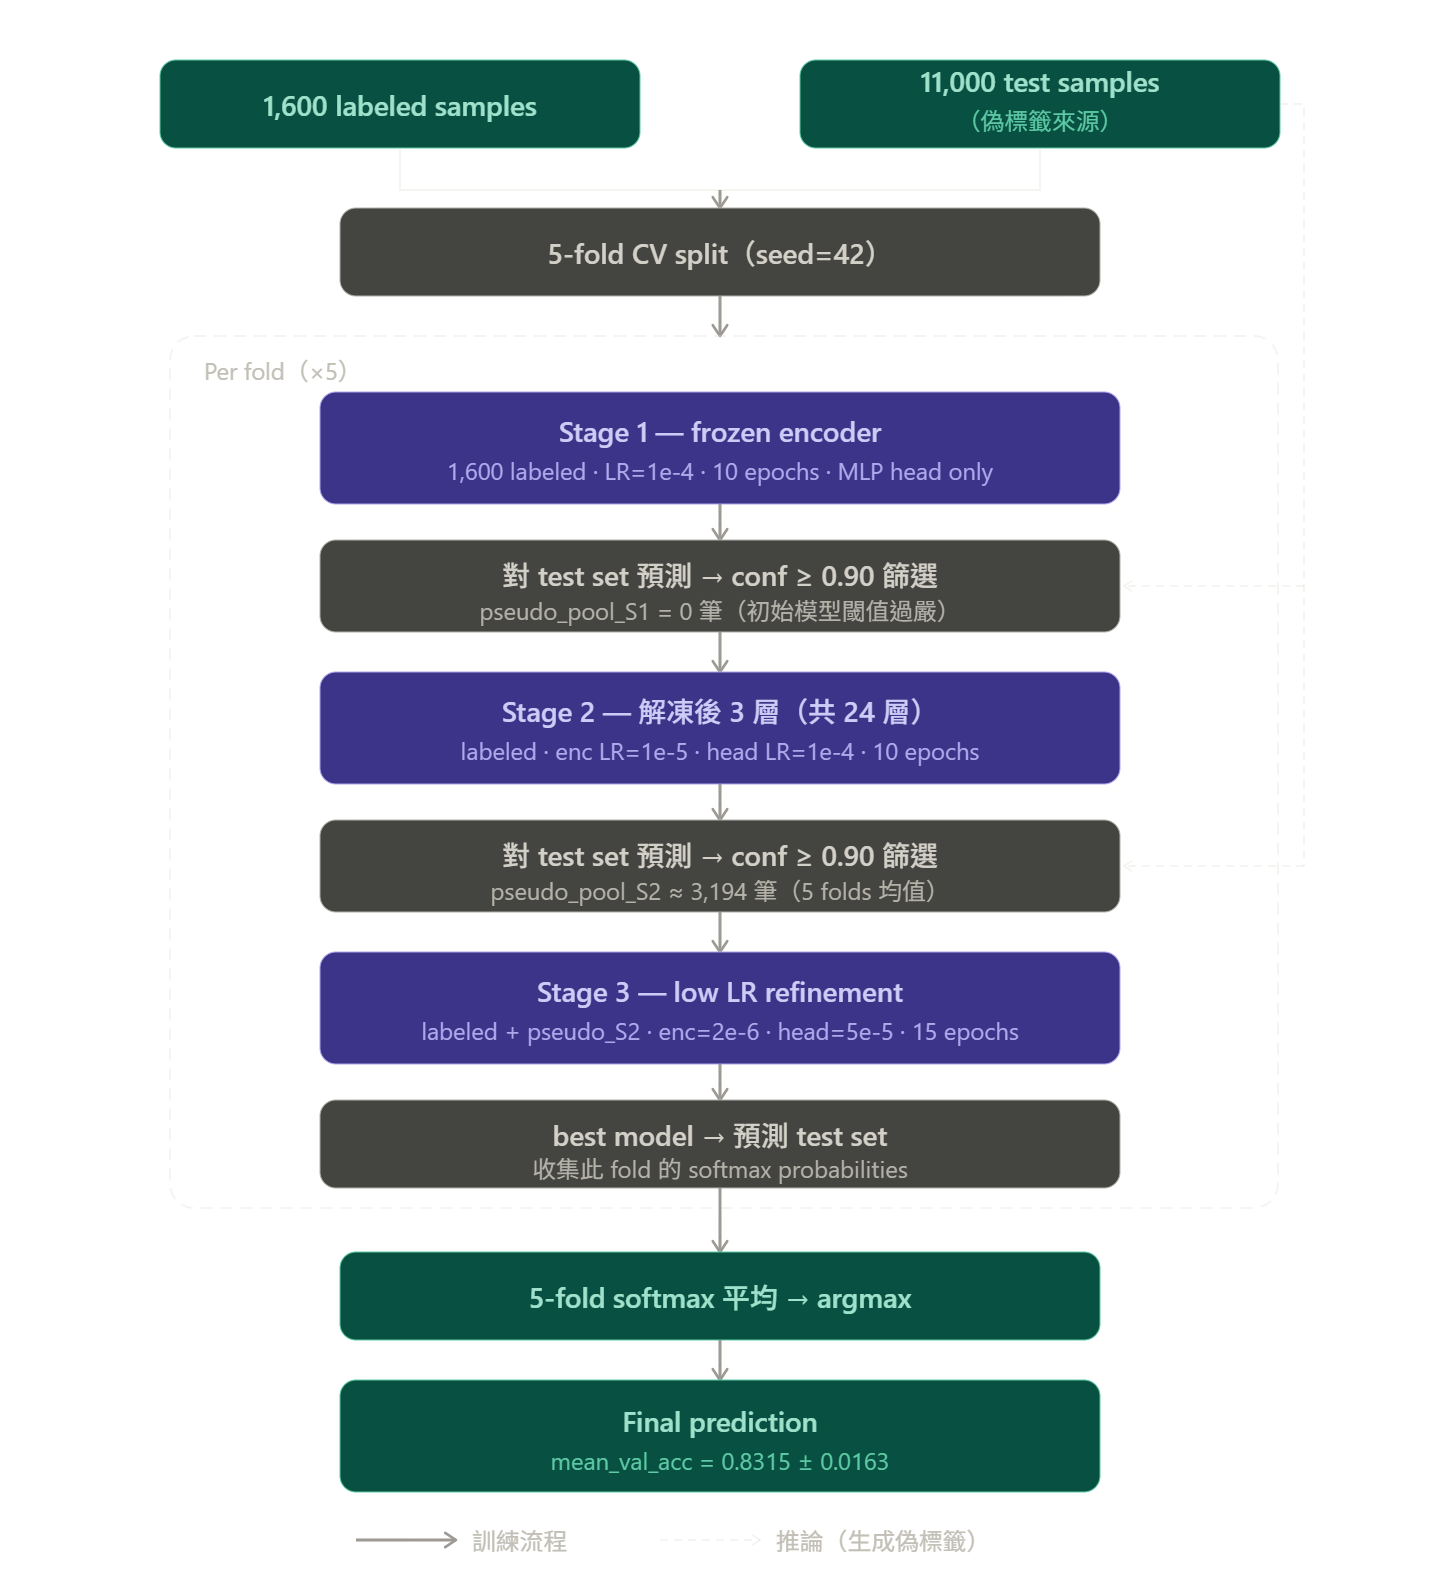
\includegraphics[width=\columnwidth]{exp09-05.png}
  \caption{EXP01 pipeline: three-stage self-training with progressive
    encoder unfreezing (exp09-05).}
  \label{fig:exp01}
\end{figure}

\begin{figure}[h]
  \centering
  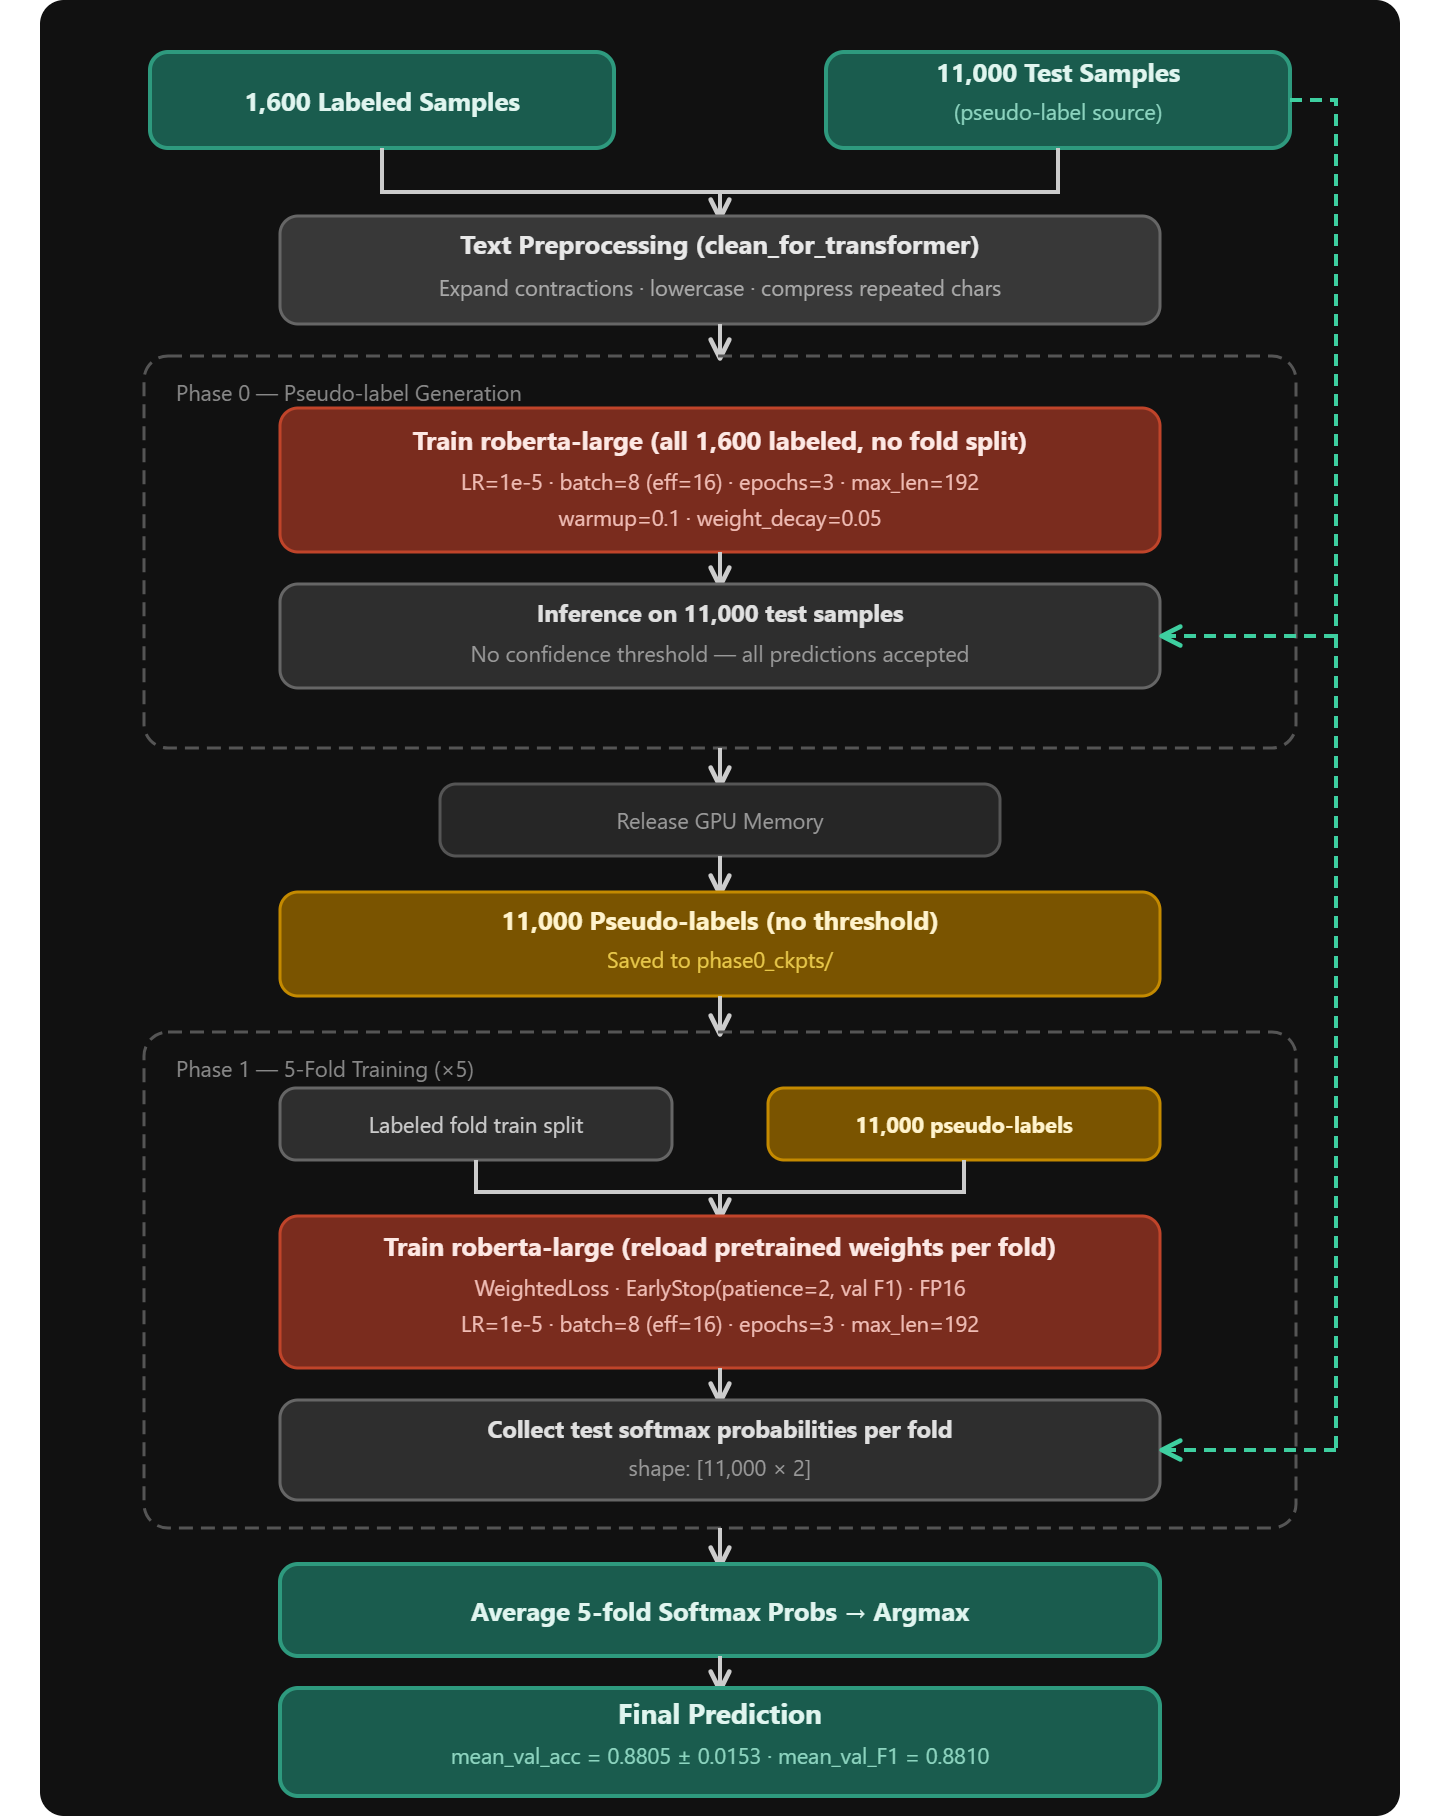
\includegraphics[width=\columnwidth]{exp11-01.png}
  \caption{EXP02 pipeline: two-stage full pseudo-label strategy with
    balanced class weights and Early Stopping (exp11-01).}
  \label{fig:exp02}
\end{figure}

%% ════════════════════════════════════════════════════════════════════════════════
\section{Methodology}

\subsection{Experiment Overview}

This study designs two semi-supervised training schemes centered on
pseudo-labeling, both using RoBERTa-large as the backbone and evaluated
with 5-fold cross-validation. The core concept of EXP01 is
\emph{Progressive Unfreezing} combined with \emph{Self-training}:
through three training stages, the encoder is first frozen to build a
stable classification head, then the last three encoder layers are
progressively unfrozen, and pseudo-labels filtered by confidence
threshold are incrementally added to the training data. EXP02 adopts a
more direct \emph{full pseudo-label strategy}: Phase~0 generates 11,000
pseudo-labels from full test-set predictions by the warm-up model, which
are then directly incorporated in the 5-fold training of Phase~1, with
balanced class weights and Early Stopping controlling training stability.

To ensure reproducibility, both schemes fix the random seed
(\texttt{seed~=~42}) and call \texttt{set\_seed()} before training.
EXP01 additionally sets \texttt{cudnn.deterministic~=~True} and
\texttt{cudnn.benchmark~=~False} to eliminate non-determinism in CUDA
convolution operations; EXP02 passes the seed through HuggingFace
\texttt{TrainingArguments(seed=42)} into the Trainer framework. The
5-fold splits in both schemes use
\texttt{StratifiedKFold(random\_state=42)} to ensure consistent fold
assignments across runs.

\subsection{Data Preprocessing}

EXP01 performs no text cleaning and feeds raw text directly to the
model. EXP02 applies text normalization before loading data, correcting
common split-contraction noise in the dataset. EXP02 therefore uses
regular expressions to restore common negative contractions, personal
pronoun contractions, and auxiliary verb contractions to their full
forms, converts all text to lowercase to eliminate case differences, and
collapses repeated characters (e.g., \texttt{"loooove"}$\to$\texttt{"loove"})
to reduce surface noise. Detailed rules are listed in Appendix~C.

\subsection{Model Selection}

Early experiments compared two candidate backbone models:
\texttt{siebert/sentiment-roberta-large-english}~\cite{hartmann2023} and
\texttt{roberta-large}~\cite{liu2019roberta}. The former is a fine-tuned
version of RoBERTa-large on large-scale sentiment classification datasets;
the latter is a general-purpose pre-trained model trained with Masked
Language Modeling (MLM), with a more complete and malleable language
representation space.

\begin{table}[h]
\centering
\caption{Backbone model comparison (preliminary runs)}
\label{tab:backbone}
\resizebox{\columnwidth}{!}{%
\begin{tabular}{lcc}
\toprule
\textbf{Item} & \textbf{siebert (run02)} & \textbf{roberta-large (run05)} \\
\midrule
Pre-training   & Sentiment-specialized & General-purpose MLM \\
Parameters     & $\sim$355M  & $\sim$355M \\
Mean val acc   & \textbf{0.8565} (std=0.0094) & 0.8315 (std=0.0163) \\
Kaggle public  & 0.74490     & \textbf{0.77465} \\
Val$\to$pub.\ gap & $\sim$0.1115 (overfit) & $\sim$0.057 (better) \\
Pipeline compat. & Low       & High \\
\bottomrule
\end{tabular}}
\end{table}

As shown in Table~\ref{tab:backbone}, siebert (run02) achieved a higher
validation accuracy (0.8565) but only scored 0.74490 on Kaggle public,
a gap of 0.1115, indicating severe overfitting on this small dataset.
In contrast, roberta-large (run05) slightly reduced validation accuracy
to 0.8315 but substantially improved the Kaggle public score to 0.77465,
narrowing the val-to-public gap to 0.057. This result confirms that
roberta-large's intact language representation space is better suited
as the backbone for this study's custom training pipeline; therefore it
was adopted as the shared backbone for both schemes.

\subsection{EXP01 --- Self-Training + Progressive Encoder Unfreezing}

The core design philosophy of EXP01 is to reduce overfitting risk
through a ``stabilize first, then expand'' progressive strategy. The
overall training is divided into three stages, with pseudo-labels
generated from model predictions on the test set between stages. All
stages are executed independently under a 5-fold cross-validation
framework, with final predictions being the average softmax
probabilities of the best model from each fold.

\subsubsection{Model Architecture}
EXP01 adds a custom classification head on top of the roberta-large
encoder:
\[
  \text{Linear}(1024{\to}64) \to \text{ReLU} \to \text{Dropout}(0.1)
  \to \text{Linear}(64{\to}2)
\]
The intermediate layer compresses the 1,024-dimensional encoder output
to 64 dimensions. This lightweight bottleneck design is especially
critical in Stage~1 when the encoder is frozen, limiting trainable
parameters to prevent memorization of training noise in a low-data
setting.

\subsubsection{Training Pipeline (3 Stages $\times$ 5-fold CV)}

\paragraph{Stage~1 --- Frozen Encoder.}
Stage~1 freezes all roberta-large encoder layers and trains only the
classification head on 1,600 labeled samples (LR~=~1e-4, epochs~=~10,
max\_length~=~128, label smoothing~=~0.1, warmup ratio~=~0.1). This
stage serves two purposes: (1)~to build a stable initial classifier
without corrupting pre-trained representations; (2)~to predict the
11,000 test samples and filter those with softmax confidence
$\geq$~0.90 as the first batch of pseudo-labels
(\texttt{pseudo\_pool\_S1}).

Due to the strict 0.90 threshold being too demanding for the Stage~1
initial model, \texttt{pseudo\_pool\_S1} was \textbf{0 samples} for all
folds. Stage~2 therefore effectively begins training on pure labeled
data.

\paragraph{Stage~2 --- Unfreeze Last 3 Layers.}
Stage~2 unfreezes the last 3 Transformer encoder layers (of 24~total)
and fine-tunes with layer-wise learning rates (encoder LR~=~1e-5, head
LR~=~1e-4, epochs~=~10, max\_length~=~128, label smoothing~=~0.1,
warmup ratio~=~0.1). The encoder LR is set to 1/10 of the head LR,
allowing upper encoder representations to gradually adapt to the
sentiment distribution while avoiding catastrophic forgetting. Upon
completion, predictions are made on all 11,000 test samples and those
with confidence $\geq$~0.90 are selected as \texttt{pseudo\_pool\_S2}
for Stage~3.

\begin{table}[h]
\centering
\caption{Pseudo-label volume from Stage~2 per fold}
\label{tab:pseudo_s2}
\begin{tabular}{cc}
\toprule
\textbf{Fold} & \textbf{n\_pseudo\_S2} \\
\midrule
0 & 3,040 \\
1 & 3,036 \\
2 & 2,879 \\
3 & 3,563 \\
4 & 3,451 \\
\midrule
\textbf{Mean} & \textbf{3,193.8} \\
\bottomrule
\end{tabular}
\end{table}

\paragraph{Stage~3 --- Low-LR Refinement.}
Stage~3 uses the best weights from Stage~2 as a warm-start, applying
lower learning rates (encoder LR~=~2e-6, head LR~=~5e-5, epochs~=~15,
warmup ratio~=~0.05) for final refinement. Training data consists of
1,600 labeled samples plus \texttt{pseudo\_pool\_S2} (average
$\approx$3,194 samples per fold). No new pseudo-labels are generated.

\subsubsection{Pseudo-label Strategy}
EXP01 uses confidence-threshold filtering (confidence $\geq$~0.90),
maintaining pseudo-label quality. However, the overly strict Stage~1
threshold resulted in \texttt{pseudo\_pool\_S1}~=~0 for all folds,
making Stage~2 equivalent to training on labeled data only. Effective
pseudo-label incorporation was not achieved until after Stage~2,
providing an average of $\approx$3,194 additional training samples per
fold.

\subsubsection{Ensemble}
Each fold independently completes three training stages and outputs
softmax probability distributions on the test set using its Stage~3
best model. Final predictions are obtained by averaging the softmax
probabilities sample-wise across all 5~folds, then converting to class
labels via argmax.

\subsection{EXP02 --- Phase~0 Pseudo-label + 5-fold Ensemble}

The core design philosophy of EXP02 is to fully utilize the 11,000
unlabeled test samples with minimal complexity. Phase~0 trains a
warm-up model on all labeled data and generates full pseudo-labels;
Phase~1 trains a 5-fold model using each fold's labeled data plus all
pseudo-labels, with balanced class weights and Early Stopping.

\subsubsection{Model Architecture}
EXP02 loads roberta-large via HuggingFace
\texttt{AutoModelForSequenceClassification}, using the default
\texttt{RobertaClassificationHead}:
\[
  \text{Drop} \to \text{Linear}(1024{\to}1024) \to \text{Tanh}
  \to \text{Drop} \to \text{Linear}(1024{\to}2)
\]
trained with FP16 mixed precision. Compared to EXP01's custom
lightweight head, EXP02 maintains the default full-dimension head and
uses the HuggingFace Trainer framework, reducing the complexity of
custom code.

\subsubsection{Training Pipeline (2 Phases $\times$ 5-fold CV)}

\paragraph{Phase~0 --- Pseudo-label Generation.}
Phase~0 trains roberta-large on all 1,600 labeled samples without fold
splitting (LR~=~1e-5, batch size~=~8, gradient accumulation~=~2,
effective batch~=~16, epochs~=~3, max\_length~=~192, warmup
ratio~=~0.1, weight decay~=~0.05). After training, predictions are made
on all 11,000 test samples \emph{without} a confidence threshold; all
predictions are directly used as pseudo-labels.

\paragraph{Phase~1 --- 5-fold Training.}
Phase~1 trains each fold using \texttt{labeled\_fold\_train}
($\approx$1,280 samples) plus the 11,000 pseudo-labels generated in
Phase~0 (same hyperparameters). Training uses balanced class weights
(\texttt{WeightedTrainer}) and \texttt{EarlyStoppingCallback}
(patience~=~2, monitoring val F1).

\subsubsection{Pseudo-label Strategy}
EXP02 discards confidence-threshold filtering and directly incorporates
all 11,000 full predictions. The core rationale is that while focusing
on high-confidence samples ensures pseudo-label quality, overly strict
filtering under severely data-scarce conditions actually limits the
augmentation benefit. Class weights combined with Early Stopping
mitigate the negative impact of lower-quality pseudo-labels.

\subsubsection{Ensemble}
Each fold independently completes Phase~1 training and outputs softmax
probability distributions on the test set using its best checkpoint.
Final predictions are obtained by averaging sample-wise softmax
probabilities across all 5~folds, then converting to class labels via
argmax.

%% ════════════════════════════════════════════════════════════════════════════════
\section{Experiments \& Results}

\subsection{Shared Settings}

\begin{table}[h]
\centering
\caption{Shared experimental settings}
\label{tab:shared}
\resizebox{\columnwidth}{!}{%
\begin{tabular}{lcc}
\toprule
\textbf{Item} & \textbf{EXP01} & \textbf{EXP02} \\
\midrule
Base model       & roberta-large   & roberta-large \\
Seed             & 42              & 42 \\
CV               & 5-fold Stratified & 5-fold Stratified \\
Primary metric   & Accuracy        & Accuracy + F1 \\
Class balancing  & ---             & Balanced weights \\
Early stopping   & None            & patience=2 (val F1) \\
Label smoothing  & 0.1             & None \\
\bottomrule
\end{tabular}}
\end{table}

As shown in Table~\ref{tab:shared}, both schemes use roberta-large as
the backbone, 5-fold Stratified CV as the validation framework, and fix
the random seed (seed~=~42) for reproducibility. The main differences
lie in class imbalance handling, Early Stopping configuration, and Label
Smoothing usage.

\subsection{EXP01 Per-Fold Results}

\begin{table}[h]
\centering
\caption{EXP01 per-fold validation results}
\label{tab:exp01}
\resizebox{\columnwidth}{!}{%
\begin{tabular}{ccccc}
\toprule
\textbf{Fold} & \textbf{S1 Acc} & \textbf{S2 Acc} &
\textbf{Best Val Acc} & \textbf{n\_pseudo\_S2} \\
\midrule
0 & 0.7550 & 0.8325 & 0.8325 & 3,040 \\
1 & 0.7650 & 0.8225 & 0.8425 & 3,036 \\
2 & 0.7475 & 0.7875 & 0.8000 & 2,879 \\
3 & 0.7400 & 0.8225 & 0.8375 & 3,563 \\
4 & 0.7300 & 0.8300 & 0.8450 & 3,451 \\
\midrule
\textbf{Mean} & 0.7475 & 0.8210 & \textbf{0.8315} & 3,193.8 \\
\textbf{Std}  & ---    & ---    & 0.0163  & --- \\
\bottomrule
\end{tabular}}
\end{table}

As shown in Table~\ref{tab:exp01}, EXP01's Stage~1 accuracy per fold
ranges from 0.730 to 0.765. After unfreezing the last 3 layers in
Stage~2, per-fold accuracy improved substantially (0.788--0.833), with
a final mean Best Val Acc of 0.8315 (std~=~0.0163). Notably,
\texttt{pseudo\_pool\_S1}~=~0 for all folds; pseudo-labels were only
generated from Stage~2, providing an average of $\approx$3,194
additional training samples per fold. Fold~2 performed noticeably lower
(0.8000), resulting in the relatively larger overall standard deviation.
Kaggle public score: 0.77465, private score: 0.77815.

\subsection{EXP02 Per-Fold Results}

\begin{table}[h]
\centering
\caption{EXP02 per-fold validation results}
\label{tab:exp02}
\begin{tabular}{cccc}
\toprule
\textbf{Fold} & \textbf{Val Acc} & \textbf{Val Loss} & \textbf{Val F1} \\
\midrule
0 & 0.8725 & 0.6221 & 0.8765 \\
1 & 0.9025 & 0.4379 & 0.9051 \\
2 & 0.8650 & 0.6580 & 0.8670 \\
3 & 0.8675 & 0.4105 & 0.8630 \\
4 & 0.8950 & 0.4358 & 0.8934 \\
\midrule
\textbf{Mean} & \textbf{0.8805} & --- & \textbf{0.8810} \\
\textbf{Std}  & 0.0153          & --- & --- \\
\bottomrule
\end{tabular}
\end{table}

As shown in Table~\ref{tab:exp02}, EXP02's per-fold validation accuracy
ranges from 0.865 to 0.903, with a mean Val Acc of 0.8805
(std~=~0.0153) and mean Val F1 of 0.8810. Fold~1 performed best
(0.9025), while Fold~2 was relatively lower (0.8650) but still
outperformed all EXP01 folds. The overall standard deviation (0.0153)
is slightly lower than EXP01 (0.0163), indicating more consistent
performance. Kaggle public score: 0.77988, private score: 0.79864.

\subsection{Overall Comparison}

\begin{table}[h]
\centering
\caption{Comprehensive comparison of EXP01 vs.\ EXP02}
\label{tab:compare}
\resizebox{\columnwidth}{!}{%
\begin{tabular}{lcc}
\toprule
\textbf{Item} & \textbf{EXP01} & \textbf{EXP02} \\
\midrule
Mean Val Acc           & 0.8315  & \textbf{0.8805} \\
Val Acc Std            & 0.0163  & \textbf{0.0153} \\
Mean Val F1            & ---     & \textbf{0.8810} \\
Kaggle public score    & 0.77465 & \textbf{0.77988} \\
Kaggle private score   & 0.77815 & \textbf{0.79864} \\
Pseudo-label volume    & $\sim$3,194 (Stage~2) & 11,000 (full) \\
Conf.\ threshold  & 0.90    & None \\
Encoder unfreezing     & Last 3 layers (S2+) & Full (Ph.\,0\,\&\,1) \\
Training stages        & $3\times5$ folds & $2\times5$ folds \\
\bottomrule
\end{tabular}}
\end{table}

As shown in Table~\ref{tab:compare}, EXP02 outperforms EXP01 across all
metrics. Validation accuracy improved by $\approx$4.9~pp (0.8805
vs.~0.8315), and Kaggle private score improved by $\approx$2~pp
(0.79864 vs.~0.77815). This result indicates that the two-stage
strategy of full pseudo-labels with class weighting and Early Stopping
outperforms the three-stage strategy of confidence-filtered pseudo-labels
with progressive unfreezing in this low-resource setting. In EXP01, the
overly strict Stage~1 threshold (\texttt{pseudo\_pool\_S1}~=~0)
effectively prevented pseudo-label incorporation before Stage~2,
undermining the intended benefit of the multi-stage design.

%% ════════════════════════════════════════════════════════════════════════════════
\section{Conclusion and Future Work}

This study establishes a reproducible low-resource sentiment
classification pipeline. Under a fixed validation framework, two
RoBERTa-large-based pseudo-labeling schemes are designed, compared, and
evaluated based on mean accuracy, F1, and cross-fold stability. EXP01's
overly strict Stage~1 confidence threshold (\texttt{pseudo\_pool\_S1}~=~0)
undermined the multi-stage design, ultimately achieving mean Val
Acc~=~0.8315 and private score~=~0.77815. EXP02's simpler two-stage
strategy---full pseudo-label incorporation with balanced class weights
and Early Stopping---achieved mean Val Acc~=~0.8805 and private
score~=~0.79864, outperforming EXP01 on all metrics. These results
confirm that in low-resource NLP classification tasks, the quality of
the pre-trained backbone and the robustness of the augmentation strategy
are more decisive than the complexity of the training pipeline.

Future work will focus on four directions: (1)~adjust EXP01 Stage~1
threshold (e.g., 0.80) to achieve \texttt{pseudo\_pool\_S1}~$>$~0;
(2)~compare pseudo-label effects with and without confidence filtering
in EXP02; (3)~explore other BERT-family models such as DeBERTa-v3;
(4)~add label smoothing to EXP02 to further improve generalization in
low-resource settings.

%% ── References ───────────────────────────────────────────────────────────────
\section*{References}
\begingroup
\renewcommand{\section}[2]{}
\begin{thebibliography}{9}
\small
\bibitem{liu2019roberta}
Y.~Liu, M.~Ott, N.~Goyal, J.~Du, M.~Joshi, D.~Chen, O.~Levy,
M.~Lewis, L.~Zettlemoyer, and V.~Stoyanov,
``RoBERTa: A Robustly Optimized BERT Pretraining Approach,''
\textit{arXiv preprint arXiv:1907.11692}, 2019.

\bibitem{hartmann2023}
J.~Hartmann, M.~Heitmann, C.~Siebert, and C.~Schamp,
``More than a Feeling: Accuracy and Application of Sentiment Analysis,''
\textit{International Journal of Research in Marketing},
vol.~40, no.~1, pp.~75--87, 2023.
\end{thebibliography}
\endgroup

%% ── Appendix ─────────────────────────────────────────────────────────────────
\appendix

\section{EXP01 Full Hyperparameter Settings}

\noindent\textbf{Model Architecture}

\vspace{3pt}
\noindent\resizebox{\columnwidth}{!}{%
\begin{tabular}{ll}
\toprule
\textbf{Item} & \textbf{Setting} \\
\midrule
Base model & roberta-large \\
Head & Linear(1024$\to$64)$\to$ReLU$\to$Drop(0.1)$\to$Lin(64$\to$2) \\
Precision & FP32 \\
\bottomrule
\end{tabular}}

\vspace{6pt}
\noindent\textbf{Stage 1 / Stage 2 / Stage 3}

\vspace{3pt}
\noindent\resizebox{\columnwidth}{!}{%
\begin{tabular}{lccc}
\toprule
\textbf{Hyperparam.} & \textbf{Stage 1} & \textbf{Stage 2} & \textbf{Stage 3} \\
\midrule
Data             & Labeled (1,600) & Lab+pseudo\_S1 & Lab+pseudo\_S2 \\
Encoder          & Frozen          & Last 3 unfrozen & All \\
LR (encoder)     & ---             & 1e-5           & 2e-6 \\
LR (head)        & 1e-4            & 1e-4           & 5e-5 \\
Batch size       & 32              & 32             & 32 \\
Epochs           & 10              & 10             & 15 \\
Max length       & 128             & 128            & 128 \\
Label smoothing  & 0.1             & 0.1            & 0.1 \\
Warmup ratio     & 0.1             & 0.1            & 0.05 \\
Conf.\ threshold & 0.90            & 0.90           & --- \\
\bottomrule
\end{tabular}}

\section{EXP02 Full Hyperparameter Settings}

\noindent\textbf{Model Architecture}

\vspace{3pt}
\noindent\resizebox{\columnwidth}{!}{%
\begin{tabular}{ll}
\toprule
\textbf{Item} & \textbf{Setting} \\
\midrule
Base model & roberta-large \\
Head & HF default RobertaClassificationHead \\
Precision & FP16 (mixed precision) \\
\bottomrule
\end{tabular}}

\vspace{6pt}
\noindent\textbf{Phase 0 / Phase 1}

\vspace{3pt}
\noindent\resizebox{\columnwidth}{!}{%
\begin{tabular}{lcc}
\toprule
\textbf{Hyperparam.} & \textbf{Phase 0} & \textbf{Phase 1} \\
\midrule
Data               & All labeled (1,600) & fold\_train + 11,000 pseudo \\
LR                 & 1e-5              & 1e-5 \\
Batch size         & 8                 & 8 \\
Grad.\ accum.      & 2 (eff.\ 16)      & 2 (eff.\ 16) \\
Epochs             & 3                 & 3 (+ EarlyStop) \\
Early stop         & ---               & patience=2 (val F1) \\
Max length         & 192               & 192 \\
Warmup ratio       & 0.1               & 0.1 \\
Weight decay       & 0.05              & 0.05 \\
Class balancing    & ---               & Balanced (WeightedTrainer) \\
Conf.\ threshold   & None (all 11,000) & --- \\
Seed / n\_folds    & 42 / ---          & 42 / 5 \\
\bottomrule
\end{tabular}}

\clearpage
\section{\texttt{clean\_text} Contraction Correction Rules (EXP02)}

\begin{table}[h]
\centering
\caption{Regex contraction correction rules}
\label{tab:contraction}
\resizebox{\columnwidth}{!}{%
\begin{tabular}{ll}
\toprule
\textbf{Original form} & \textbf{Corrected form} \\
\midrule
\texttt{(\textbackslash{}w+) t}  & \texttt{not} (e.g.\ \texttt{can t}$\to$\texttt{cannot}) \\
\texttt{i m}                     & \texttt{i am} \\
\texttt{it s}                    & \texttt{it is} \\
\texttt{(\textbackslash{}w+) re} & \texttt{ are} \\
\texttt{(\textbackslash{}w+) ve} & \texttt{ have} \\
\texttt{(\textbackslash{}w+) ll} & \texttt{ will} \\
\bottomrule
\end{tabular}}
\end{table}

\end{document}
